\documentclass{article}

\usepackage[preprint]{neurips_2024}

\usepackage[utf8]{inputenc}
\usepackage[T1]{fontenc}
\usepackage{hyperref}
\usepackage{url}
\usepackage{booktabs}
\usepackage{amsfonts}
\usepackage{xcolor}
\usepackage{graphicx}
\usepackage{enumitem}
\usepackage{multirow}

\title{Agent RAGLAW: Agentic Legal RAG with Adaptive Planning}

\author{%
  Hamza Iqbal \\
  Washington University in St.\ Louis \\
  \texttt{hiqbal@wustl.edu}
  \And
  Hanson Li \\
  Washington University in St.\ Louis \\
  \texttt{hanson.l@wustl.edu}
  \And
  Josh Li \\
  Washington University in St.\ Louis \\
  \texttt{josh.l@wustl.edu}
}

\begin{document}

\maketitle

\begin{abstract}
Standard retrieval-augmented generation (RAG) pipelines use a single query--retrieve--generate pass, which often fails on legal questions that require synthesizing multiple doctrines or applying abstract rules to specific fact patterns. We present an agentic legal RAG system built on LangGraph that replaces single-shot retrieval with an adaptive plan-and-solve loop: a classifier generates a multi-step research plan, an executor retrieves and synthesizes evidence per step with diversified multi-query retrieval and cross-encoder reranking, an evaluator grades retrieval quality, and a replanner adaptively refines the plan based on accumulated evidence. We evaluate on 100 randomly sampled Bar Exam QA multiple-choice questions using Gemma~3 27B and DeepSeek Reasoner as backbone LLMs. Our results reveal that the agentic pipeline underperforms the direct LLM baseline for both models (45\% vs.\ 57\% for Gemma; 72\% vs.\ 92\% for DeepSeek), highlighting that structured retrieval scaffolding can constrain strong reasoners while also revealing critical sensitivity to prompt engineering in the query generation stage.
\end{abstract}

%------------------------------------------------------------------
\section{Introduction}
%------------------------------------------------------------------

Legal question answering is a challenging domain for retrieval-augmented generation (RAG). Legal answers must be both correct \emph{and} precise---small omissions or mischaracterizations can change meaning entirely. Furthermore, the relevant legal principles (exceptions, narrow holdings, definitional clauses) are often spread across multiple passages, requiring a system to identify and synthesize several pieces of evidence rather than relying on a single retrieved chunk.

Standard single-shot RAG pipelines---where the user query is sent directly to a retriever, the top-$k$ passages are concatenated into a prompt, and an LLM generates an answer---struggle with this setting for two reasons. First, a single query may not capture all facets of a multi-concept legal question (e.g., a torts question involving duty, breach, causation, \emph{and} superseding cause). Second, without feedback on retrieval quality, the system cannot detect when it has retrieved irrelevant passages and needs to reformulate its search.

We propose an \textbf{agentic legal RAG} system that addresses these limitations through adaptive multi-step planning. Rather than a single retrieval pass, our system: (i)~classifies the complexity of the query, (ii)~generates a structured research plan decomposing the question into retrieval sub-steps, (iii)~executes each step with diversified multi-query retrieval and cross-encoder reranking, (iv)~evaluates retrieval quality and adaptively replans when evidence is insufficient, and (v)~synthesizes a citation-grounded answer from the accumulated evidence.

We evaluate on the Bar Exam QA dataset \cite{barexamqa}, a collection of multiple-choice bar exam questions with gold passage annotations. Our preliminary results on 100 questions reveal surprising findings: the agentic pipeline does not outperform a direct LLM baseline for either model tested, though the gap is much smaller for the weaker model (Gemma: 45\% vs.\ 57\%) than for the strong reasoner (DeepSeek: 72\% vs.\ 92\%). These results suggest that agentic scaffolding may be most valuable for models that lack sufficient parametric legal knowledge, while the overhead of structured retrieval can actively hinder strong reasoners. We also find that prompt engineering at the query generation stage is a critical---and under-appreciated---bottleneck.

%------------------------------------------------------------------
\section{Related Work}
%------------------------------------------------------------------

\textbf{Legal Benchmarks and Datasets.}
LegalBench~\cite{guha2023legalbench} provides a broad evaluation framework spanning 162 tasks that test distinct legal reasoning capabilities. Bar Exam QA~\cite{barexamqa} provides multiple-choice bar exam questions paired with gold passage annotations from a corpus of approximately 686K passages covering seven subjects (Constitutional Law, Contracts/UCC, Criminal Law/Procedure, Evidence, Real Property, Torts, and Civil Procedure), enabling evaluation of both retrieval accuracy and end-to-end QA performance. LegalRetrievalBench~\cite{zheng2025legalretrievalbench} introduces a reasoning-focused retrieval benchmark that tests whether systems can identify passages relevant to complex legal reasoning chains, rather than simple keyword-based matching. Our work uses Bar Exam QA as the primary evaluation dataset.

\textbf{Agentic RAG and Multi-Step Retrieval.}
The idea of using LLM agents to decompose complex questions into sub-queries has been explored in several recent systems. Self-RAG~\cite{selfrag2024} trains models to adaptively retrieve passages and critique their own generations, deciding when retrieval is needed and whether the generated output is supported by the retrieved evidence. CRAG (Corrective RAG)~\cite{crag2024} introduces a lightweight retrieval evaluator that triggers web search as a fallback when initial retrieval confidence is low. Adaptive-RAG~\cite{adaptiverag2024} classifies query complexity to dynamically select between single-step and multi-step retrieval strategies, similar to our classify-and-plan approach. Our system builds on these ideas by combining query complexity classification with an explicit planning table that decomposes multi-hop questions into sequential retrieval sub-steps, with adaptive replanning after each step.

\textbf{Query Rewriting and Diversification.}
Query rewriting is a well-established technique for improving retrieval in RAG systems. MultiQueryRetriever~\cite{langchain2023} generates multiple query variants to capture different phrasings of the same information need. HyDE (Hypothetical Document Embeddings)~\cite{hyde2023} generates a hypothetical answer and uses it as the retrieval query, achieving strong performance when the target corpus style differs from the query style. Our system uses a multi-query approach where the LLM generates a primary retrieval query plus two alternatives using different legal terminology, which are pooled and reranked with a cross-encoder to bridge terminological gaps between user questions and corpus passages.

\textbf{Cross-Encoder Reranking.}
Two-stage retrieval with cross-encoder reranking has become standard practice for improving retrieval precision~\cite{nogueira2019passage}. The bi-encoder (embedding model) efficiently retrieves a large candidate pool, and the cross-encoder evaluates each query-passage pair with full attention, producing more accurate relevance scores. Our system uses \texttt{cross-encoder/ms-marco-MiniLM-L-6-v2}~\cite{reimers2019sentencebert} for reranking, which also provides the confidence scores used by the evaluator to determine whether retrieval was sufficient.

%------------------------------------------------------------------
\section{Proposed Framework}
%------------------------------------------------------------------

Our system is implemented as a state machine in LangGraph~\cite{langgraph} with an adaptive plan-execute-evaluate loop. The architecture has evolved during development: the initial design (Figure~\ref{fig:architecture}) used 9~nodes with separate classifier, planner, and memory writeback stages; iterative simplification merged the classifier and planner into a single node and removed the memory writeback (which cached answers but served stale results), yielding the current 7-node design. Below we describe each component of the current system.

\begin{figure}[t]
\centering
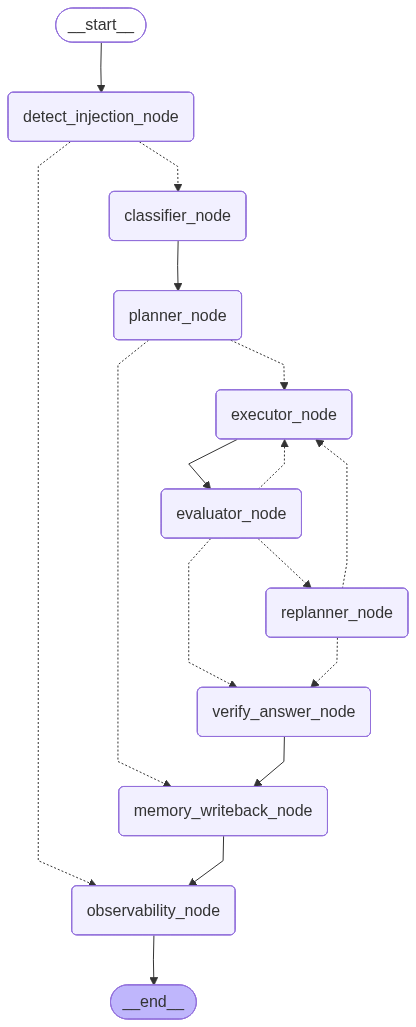
\includegraphics[width=0.38\textwidth]{agentic_langgraph_graph.png}
\caption{Initial 9-node LangGraph architecture. The current system merges classifier\_node and planner\_node into a single classify\_and\_plan node, and removes memory\_writeback\_node, yielding 7 nodes total.}
\label{fig:architecture}
\end{figure}

\subsection{Query Classification and Planning}

Given an input query, a single LLM call classifies it as \texttt{simple} (single legal concept, one retrieval step) or \texttt{multi\_hop} (multiple concepts requiring sequential retrieval). The same call generates a \textbf{planning table}---a structured JSON array where each entry specifies a research phase, a retrieval question, and an expected answer. For multiple-choice questions, the answer choices are stripped before planning to prevent the LLM from anchoring on specific options rather than conducting unbiased research.

A key design rule is that retrieval questions must be \textbf{doctrine-level}: they target abstract legal principles rather than fact-specific scenarios. For example, given a question about a mechanic who negligently inspected brakes, the retrieval question should be ``What are the elements of negligent inspection?'' rather than ``What is the standard of care for a mechanic inspecting brakes?'' This ensures that queries match the corpus format, which contains textbook-style legal rules rather than case-specific analyses.

\subsection{Executor: Multi-Query Retrieval and Synthesis}

For each pending step in the planning table, the executor performs three operations:

\begin{enumerate}[leftmargin=*,nosep]
    \item \textbf{Query rewriting}: An LLM call transforms the retrieval question into a primary query plus two alternatives using different legal terminology (e.g., ``wrongful termination'' vs.\ ``employment at-will discharge''). This bridges terminological gaps between the query and corpus.
    \item \textbf{Multi-query retrieval}: All three queries are submitted to the vector store (ChromaDB with Alibaba-NLP/gte-large-en-v1.5 embeddings, 1024 dimensions). The bi-encoder over-retrieves $4\times$ candidates per query, the results are pooled and deduplicated, and a cross-encoder (\texttt{ms-marco-MiniLM-L-6-v2}) reranks the full pool against the primary query, selecting the top 5 passages. Passages retrieved in prior steps are excluded via an \texttt{exclude\_ids} parameter to ensure cross-step diversity.
    \item \textbf{Synthesis}: An LLM call synthesizes the retrieved passages into a cited answer with inline \texttt{[Source~N]} references. An anti-fabrication rule instructs the model to only state facts present in the evidence passages.
\end{enumerate}

\subsection{Evaluator}

The evaluator grades each completed step by comparing the cross-encoder confidence score against a configurable threshold. Steps scoring below the threshold are marked as failed. Confidence is computed as the maximum cross-encoder logit score across the top-5 retrieved passages (positive scores indicate relevance, negative scores indicate irrelevance).

\subsection{Adaptive Replanner}

For \texttt{multi\_hop} queries, after all initially planned steps are executed, a replanner LLM call reviews the accumulated evidence and decides one of three actions:
\begin{itemize}[leftmargin=*,nosep]
    \item \texttt{next\_step}: Add a new research step targeting a gap in the evidence.
    \item \texttt{retry}: Rephrase and re-execute a failed step with a generalized query.
    \item \texttt{complete}: Evidence is sufficient to answer the question.
\end{itemize}
The replanner enforces a hard cap of 5 completed steps and a stagnation rule (3+ consecutive failures trigger early completion). A key replanner behavior is \textbf{query generalization on failure}: if a step failed because the retrieval query was too fact-specific, the replanner rewrites pending queries as abstract doctrine lookups.

\subsection{Answer Selection and Verification}

For multiple-choice questions, a dedicated MC selection call applies all accumulated research to select an answer letter. This runs once at the end, keeping per-step research unbiased (individual steps do not see the answer choices). The system also includes a prompt injection detection node (skippable for evaluation) and an observability node that logs metrics including LLM call counts, token usage, and step completion rates.

\subsection{LLM Call Budget}

The total LLM calls per query depend on the classification:
\begin{itemize}[leftmargin=*,nosep]
    \item \textbf{Simple}: 3 calls (classify/plan + query rewrite + synthesize)
    \item \textbf{Multi-hop non-MC}: 9 calls (classify/plan + $3\times$[rewrite + synthesize] + $3\times$ replan)
    \item \textbf{Multi-hop MC}: 10 calls (as above + MC selection)
\end{itemize}

%------------------------------------------------------------------
\section{Preliminary Experiment Results}
%------------------------------------------------------------------

\subsection{Experimental Setup}

\textbf{Dataset.} We evaluate on 100 randomly sampled multiple-choice questions from Bar Exam QA~\cite{barexamqa}, covering seven legal subjects. The same 100-question sample (fixed random seed) is used across all experiments for direct comparison.

\textbf{Corpus.} We index 20,000 passages from the Bar Exam QA passage corpus (out of approximately 686K total) in a ChromaDB vector store using gte-large-en-v1.5 embeddings.

\textbf{Models.} We test two backbone LLMs:
\begin{itemize}[leftmargin=*,nosep]
    \item \textbf{Gemma~3 27B} (\texttt{google/gemma-3-27b-it}), accessed via OpenRouter's free tier. A mid-size open-weight instruction-tuned model.
    \item \textbf{DeepSeek Reasoner} (\texttt{deepseek-reasoner}), a reasoning-specialized model with extended chain-of-thought capabilities.
\end{itemize}

\textbf{Baselines.} For each model, we run a \emph{baseline} evaluation: a single LLM API call with the question and answer choices, asking the model to select the correct answer with no retrieval.

\subsection{Results}

\begin{table}[t]
\centering
\caption{Bar Exam QA accuracy (100 questions). Baseline = direct LLM call with no retrieval. Agentic = full pipeline with adaptive planning and retrieval.}
\label{tab:results}
\begin{tabular}{lcccc}
\toprule
\textbf{Model} & \textbf{Baseline} & \textbf{Agentic RAG} & \textbf{$\Delta$} & \textbf{Errors} \\
\midrule
Gemma~3 27B & 57/100 (57\%) & 45/100 (45\%) & $-12\%$ & 3 \\
DeepSeek Reasoner & 92/100 (92\%) & 72/100 (72\%) & $-20\%$ & 0 \\
\bottomrule
\end{tabular}
\end{table}

Table~\ref{tab:results} shows the main results. Both models perform \emph{worse} with the agentic RAG pipeline than with direct prompting. For Gemma~3 27B, accuracy drops from 57\% to 45\%. For DeepSeek Reasoner, accuracy drops from 92\% to 72\%---a 20-point decrease despite the stronger model's superior reasoning.

\begin{table}[t]
\centering
\caption{Resource usage comparison across experimental configurations.}
\label{tab:resources}
\begin{tabular}{lccccc}
\toprule
\textbf{Configuration} & \textbf{LLM Calls} & \textbf{Avg Tokens/Q} & \textbf{Total Time} & \textbf{Cost} \\
\midrule
Gemma Baseline & 100 & --- & 719s & Free \\
Gemma Agentic & 1,310 & 11.6K in / 2.0K out & 6,057s & Free \\
DeepSeek Baseline & 100 & --- & 8,551s & \$0.81 \\
DeepSeek Agentic & 1,135 & 10.2K in / 1.9K out & 8,609s & \$0.82 \\
\bottomrule
\end{tabular}
\end{table}

Table~\ref{tab:resources} shows the resource overhead. The agentic pipeline requires $\sim$11$\times$ more LLM calls than the baseline and consumes $\sim$10--12K input tokens per query for multi-step research. Figure~\ref{fig:evals} shows the full benchmark summaries for both agentic configurations.

\begin{figure}[t]
\centering
\begin{minipage}{0.48\textwidth}
\centering
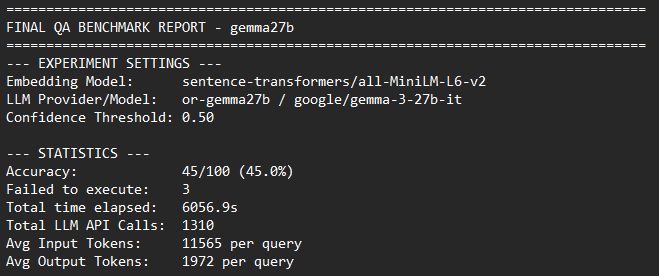
\includegraphics[width=\textwidth]{gemma_agentic_eval.png}
\end{minipage}
\hfill
\begin{minipage}{0.48\textwidth}
\centering
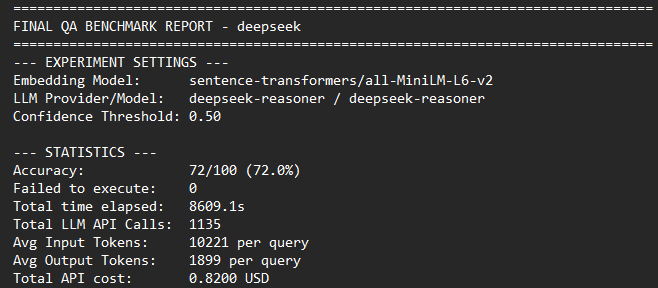
\includegraphics[width=\textwidth]{deepseek_agentic_eval.png}
\end{minipage}
\caption{Agentic pipeline benchmark results for Gemma~3 27B (left) and DeepSeek Reasoner (right). Both use the all-MiniLM-L6-v2 embedding model with a confidence threshold of 0.50.}
\label{fig:evals}
\end{figure}

\subsection{Analysis and Insights}

\textbf{Strong models are hurt by retrieval scaffolding.}
DeepSeek Reasoner achieves 92\% accuracy on bar exam questions \emph{without any retrieval}, indicating that its parametric knowledge and extended chain-of-thought reasoning already cover the legal knowledge required. Adding the retrieval pipeline drops accuracy by 20 points. We attribute this to three mechanisms: (1)~irrelevant or partially relevant passages can mislead the model away from a correct parametric answer, (2)~the multi-step structure fragments reasoning across separate LLM calls rather than allowing holistic analysis, and (3)~the rigid plan-execute loop reduces the model's autonomy. The smaller gap for Gemma ($-12\%$) versus DeepSeek ($-20\%$) is consistent with the hypothesis that the pipeline's overhead is proportional to how much the base model already knows---a model that is already near-ceiling has more to lose from noisy retrieval than one that genuinely needs external evidence.

\textbf{Query generation is the critical bottleneck.}
During development, the single most impactful change to pipeline performance was modifying the query rewriting prompt to generate \emph{doctrine-level} queries rather than fact-specific ones. For example, given a bar exam question about a mechanic installing brakes incorrectly, the initial system generated queries like ``What is the standard of care for a mechanic inspecting brakes?''---which returned no relevant passages because the corpus contains general negligence doctrine, not mechanic-specific rules. Once the prompt was updated to instruct the model to generate abstract queries like ``What are the elements of negligent inspection?'', retrieval quality improved immediately.

Critically, this issue was not identified by automated evaluation metrics or by LLM-assisted development tools used during the project---it required manual inspection of the generated queries and retrieved passages to diagnose the mismatch between query specificity and corpus format. We had invested effort in more sophisticated retrieval techniques (cross-encoder reranking, multi-query pooling, alternative embedding models) without realizing that the root cause was upstream in query generation. This highlights a fundamental limitation of agentic systems: the quality of each stage is highly sensitive to prompt engineering, and errors in upstream stages propagate through the entire pipeline in ways that downstream improvements cannot compensate for.

\textbf{Retrieval quality varies by legal subject.}
In our 8-query traced evaluation (Table~\ref{tab:trace}), Constitutional Law questions consistently scored near the confidence threshold (0.67--0.70) and produced 0 completed steps out of 3, while Torts, Contracts, and Evidence questions achieved higher confidence (0.77--0.79) and completed all steps successfully. This suggests uneven corpus coverage across subjects in our 20K-passage subset, or that Constitutional Law queries require more specialized terminology.

\begin{table}[t]
\centering
\caption{Detailed trace results on 8 representative queries (Gemma~3 27B). ``Steps'' shows completed/failed; ``Conf'' is the mean cross-encoder confidence across completed steps.}
\label{tab:trace}
\begin{tabular}{lccccc}
\toprule
\textbf{Subject} & \textbf{MC Correct?} & \textbf{Steps} & \textbf{Conf} & \textbf{Time} & \textbf{LLM Calls} \\
\midrule
Torts & Yes & 3c/0f & 0.773 & 74s & 11 \\
Contracts & Yes & 3c/0f & 0.773 & 57s & 11 \\
Crim Law & No & 3c/0f & 0.721 & 69s & 11 \\
Evidence & Yes & 3c/0f & 0.790 & 78s & 11 \\
Const Law & No & 0c/3f & --- & 91s & 11 \\
Real Property & Yes & 3c/0f & 0.775 & 74s & 11 \\
Multi-hop & n/a & 3c/0f & 0.795 & 54s & 10 \\
Out-of-corpus & n/a & 1c/0f & 0.717 & 23s & 4 \\
\bottomrule
\end{tabular}
\end{table}

\textbf{Failure mode taxonomy.}
We identify three distinct failure modes from our evaluation:
\begin{enumerate}[leftmargin=*,nosep]
    \item \textbf{Retrieval failure} (e.g., Constitutional Law): The retrieved passages do not contain the relevant doctrine. All steps fail, and the system falls back to whatever partial evidence it accumulated. The Constitutional Law trace exemplifies this---0/3 steps completed, confidence scores below threshold.
    \item \textbf{Reasoning failure} (e.g., Criminal Law): Retrieval succeeds (3/3 steps completed, confidence 0.721), but the MC selector misapplies the retrieved evidence to select the wrong answer. The research quality was adequate, but the final answer selection LLM call made an error in legal reasoning.
    \item \textbf{Scaffolding overhead}: Even when retrieval and reasoning both succeed, the pipeline can still underperform the baseline because the multi-step structure forces the model to commit to a research plan early, rather than reasoning holistically over the full question. This is most visible with DeepSeek Reasoner, which can solve most questions in a single reasoning pass.
\end{enumerate}

\textbf{Cross-step deduplication ensures passage diversity.}
One positive finding is that the \texttt{exclude\_ids} mechanism achieves 100\% unique passages across all steps in every traced query, confirming that multi-step retrieval provides genuinely diverse evidence.

%------------------------------------------------------------------
\section{Changes from Project Proposal}
%------------------------------------------------------------------

Our project proposal outlined a pipeline with query refinement, citation-grounded generation, and optional model fine-tuning. The implemented system differs in several ways:

\textbf{Iterated planning replaced single-pass planning.}
The proposal considered both an iterated approach (plan $\rightarrow$ retrieve $\rightarrow$ revise plan $\rightarrow$ retrieve again) and a single zoomed-out pass. We implemented the iterated approach via the adaptive replanner, which reviews evidence after each step and can add, modify, or remove pending steps. This proved essential for handling retrieval failures---when a step returns irrelevant passages, the replanner generalizes the query and retries.

\textbf{Architecture simplified during development.}
The initial implementation used 9 LangGraph nodes (Figure~\ref{fig:architecture}), including separate classifier and planner nodes and a memory writeback cache. Through iterative development, we merged the classifier and planner into a single node (saving one LLM call per query), removed the memory cache (which served stale answers for similar-but-distinct questions), and removed a verification LLM call that always passed (100\% pass rate across all traced queries). The current 7-node design uses 3--10 LLM calls per query depending on complexity.

\textbf{HousingQA dropped; Bar Exam QA is primary benchmark.}
The proposal listed both Bar Exam QA and HousingQA as evaluation datasets. We focused exclusively on Bar Exam QA due to its gold passage annotations (enabling retrieval-level evaluation), larger corpus, and coverage of seven legal subjects.

\textbf{Fine-tuning deferred.}
We have not pursued LoRA/QLoRA fine-tuning. The preliminary results suggest that the bottleneck is in the retrieval and query generation stages rather than in the LLM's generation quality, making pipeline improvements a higher priority than model adaptation.

\textbf{Citation grounding implemented natively.}
Rather than integrating RAGFlow~\cite{ragflow} for citations, we implemented citation-grounded generation directly through prompt engineering: the synthesis skill requires inline \texttt{[Source~N]} references and includes an anti-fabrication rule constraining the model to only state facts present in the evidence passages.

%------------------------------------------------------------------
\section{Next Steps}
%------------------------------------------------------------------

Based on our preliminary findings, we identify several directions for the remaining project:

\begin{enumerate}[leftmargin=*,nosep]
    \item \textbf{Targeted corpus expansion.} The current 20K-passage subset may be insufficient for subjects like Constitutional Law. We will evaluate whether increasing corpus size to 50--100K passages improves retrieval quality for underperforming subjects.
    \item \textbf{Ablation studies.} We plan to isolate the contribution of each pipeline component (multi-query rewriting, cross-encoder reranking, adaptive replanning) by systematically disabling them and measuring the impact on accuracy.
    \item \textbf{Weaker model evaluation.} Our hypothesis that the pipeline benefits weaker models more than strong ones needs validation with additional models (e.g., smaller LLaMA variants, Gemma~2 9B) where parametric legal knowledge is more limited.
    \item \textbf{MC selection improvement.} The MC answer selector is the final stage and receives all accumulated research at once. We will experiment with chain-of-thought selection prompts and elimination-based strategies.
    \item \textbf{Systematic error analysis.} We will categorize all 100-question failures into retrieval failures (wrong passages), reasoning failures (right passages, wrong conclusion), and scaffolding overhead (pipeline hurts a correct parametric answer) to quantify each failure mode's contribution.
\end{enumerate}

{\small
\bibliographystyle{plain}
\begin{thebibliography}{15}

\bibitem{guha2023legalbench}
N.~Guha et al.
LegalBench: A collaboratively built benchmark for measuring legal reasoning in large language models.
\emph{arXiv:2308.11462}, 2023.

\bibitem{zheng2025legalretrievalbench}
L.~Zheng et al.
A reasoning-focused legal retrieval benchmark.
\emph{arXiv:2505.03970}, 2025.

\bibitem{barexamqa}
Stanford RegLab.
Bar Exam QA.
\url{https://huggingface.co/datasets/reglab/barexam_qa}, 2025.

\bibitem{selfrag2024}
A.~Asai et al.
Self-RAG: Learning to retrieve, generate, and critique through self-reflection.
\emph{ICLR}, 2024.

\bibitem{crag2024}
S.-C.~Yan et al.
Corrective retrieval augmented generation.
\emph{arXiv:2401.15884}, 2024.

\bibitem{adaptiverag2024}
S.~Jeong et al.
Adaptive-RAG: Learning to adapt retrieval-augmented large language models through question complexity.
\emph{NAACL}, 2024.

\bibitem{langchain2023}
LangChain.
MultiQueryRetriever.
\url{https://python.langchain.com/docs/modules/data_connection/retrievers/MultiQueryRetriever}, 2023.

\bibitem{hyde2023}
L.~Gao et al.
Precise zero-shot dense retrieval without relevance labels.
\emph{ACL}, 2023.

\bibitem{nogueira2019passage}
R.~Nogueira and K.~Cho.
Passage re-ranking with BERT.
\emph{arXiv:1901.04085}, 2019.

\bibitem{reimers2019sentencebert}
N.~Reimers and I.~Gurevych.
Sentence-BERT: Sentence embeddings using Siamese BERT-networks.
\emph{EMNLP}, 2019.

\bibitem{langgraph}
LangChain.
LangGraph: Build stateful, multi-actor applications with LLMs.
\url{https://langchain-ai.github.io/langgraph/}, 2024.

\bibitem{ragflow}
Infiniflow.
RAGFlow.
\url{https://ragflow.io/docs/}, 2024.

\end{thebibliography}
}

\end{document}
